%%%%%%%%%%%%%%%%%%%%%%%%%%%%%%%%%%%%%%%%%%%%%%%%%%%%%%%%%%%%%%%%%%%%%%%%%
%%%TITLE, AUTHORS AND ABSTRACT%%%
\twocolumn[
  \begin{@twocolumnfalse}
{
\includegraphics[height=30pt]{head_foot/journal_name}\hfill\raisebox{0pt}[0pt][0pt]{
\includegraphics[height=55pt]{head_foot/RSC_LOGO_CMYK}}\\[1ex]

\includegraphics[width=18.5cm]{head_foot/header_bar}}\par
\vspace{1em}
\sffamily
\begin{tabular}{m{4.5cm} p{13.5cm} }


\includegraphics{head_foot/DOI} & \noindent\LARGE{\textbf{A metal chelate's effect on molecular recognition is not a property of the chelate}} \\
\vspace{0.3cm} & \vspace{0.3cm} \\

 & \noindent\large{Jeongyun Kim,$^{\ddag}$\textit{$^{a}$} Jin Yoo,$^{\ddag}$\textit{$^{a}$} Ku Kang$^{\ast}$\textit{$^{a}$} and Dongyoul Lee$^{\ast}$\textit{$^{b}$}} \\

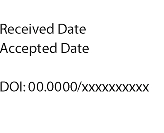
\includegraphics{head_foot/dates} & \noindent\normalsize{\sloppy\setlength{\emergencystretch}{6em}\textbf{Appending a metal chelate to a molecule that binds a biological target changes how tightly it binds. Whether that change is a property of the chelate---and therefore transferable between molecules---is assumed rather than tested, yet it is load-bearing: chelators are chosen from published comparisons and from heuristic metal--chelator matching tables. We audited it. From ten studies we assembled 106 matched affinity measurements in which one targeting molecule was conjugated to two or more chelators and assayed under a single protocol, giving 32 matched sets across five target families. Within a set the chelator alone shifts affinity by a median factor of 2.6 and by up to 25.3, while propagated measurement error accounts for only 11\% of the within-set variance. None of that signal transfers. Under leave-one-target-family-out validation an empirical chelator ranking ($R^2 = -0.250$), classical descriptors ($R^2 = -0.219$) and solvated GFN2-xTB descriptors on 27 structurally verified complexes ($R^2 = -0.340$) all do worse than assuming no effect; none orders a held-out set better than chance, and a within-set permutation test places all of them inside the no-information null. Improving the physics makes this worse rather than better: across a $2\times2$ comparison of energy term and solvation, every step that raises in-sample fit ($R^2 = 0.070 \rightarrow 0.139$) lowers held-out performance ($-0.227 \rightarrow -0.340$). Reported lipophilicity explains 7\% of the effect. What the data do contain is interaction: chelator identity crossed with target family explains $R^2 = 0.498$ against $R^2 = 0.133$ for the chelator alone. The effect is real and large but is not encoded in the chelate; it arises at a contact the isolated complex never makes. We release the dataset, geometries and analysis as an open benchmark.}}\\
\end{tabular}
 \end{@twocolumnfalse} \vspace{0.6cm}
  ]

\renewcommand*\rmdefault{bch}\normalfont\upshape
\rmfamily
\section*{}
\vspace{-1cm}

\footnotetext{\textit{$^{a}$~CBRN Defense Research Institute, Ministry of National Defense, Seoul 06796, Republic of Korea; E-mail: bisu9082@gmail.com}}
\footnotetext{\textit{$^{b}$~Korea Military Academy, Seoul 01805, Republic of Korea; E-mail: [to be supplied]}}
\footnotetext{\ddag~These authors contributed equally.}
\footnotetext{\dag~Electronic Supplementary Information (ESI) available: the complete matched affinity dataset with per-row DOI provenance (Table~S1), the optimised metal--chelate complexes with coordination verification (Table~S2), the transcribed lipophilicity values (Table~S3), the charge-artefact diagnosis and its repair (Fig.~S1), the $2\times2$ comparison of energy term and solvation (Fig.~S2), the injection power curve (Fig.~S3), and transfer under five held-out grouping schemes (Fig.~S4). See DOI: \textit{[to be assigned by RSC submission system]}.}.}
